% --------------------------------------------------------------------------- %
% Poster for the ECCS 2011 Conference about Elementary Dynamic Networks.      %
% --------------------------------------------------------------------------- %
% Created with Brian Amberg's LaTeX Poster Template. Please refer for the     %
% attached README.md file for the details how to compile with `pdflatex`.     %
% --------------------------------------------------------------------------- %
% $LastChangedDate:: 2011-09-11 10:57:12 +0200 (V, 11 szept. 2011)          $ %
% $LastChangedRevision:: 128                                                $ %
% $LastChangedBy:: rlegendi                                                 $ %
% $Id:: poster.tex 128 2011-09-11 08:57:12Z rlegendi                        $ %
% --------------------------------------------------------------------------- %
\documentclass[a0paper,landscape]{baposter}

\usepackage{relsize}		% For \smaller
\usepackage{url}			% For \url
\usepackage{epstopdf}	% Included EPS files automatically converted to PDF to include with pdflatex
\usepackage{natbib}
\usepackage{paralist}
\usepackage{wrapfig}
\usepackage[font=small,labelfont=bf]{caption}
%%% Global Settings %%%%%%%%%%%%%%%%%%%%%%%%%%%%%%%%%%%%%%%%%%%%%%%%%%%%%%%%%%%

\graphicspath{{./}}	% Root directory of the pictures 
\tracingstats=2			% Enabled LaTeX logging with conditionals

%%% Color Definitions %%%%%%%%%%%%%%%%%%%%%%%%%%%%%%%%%%%%%%%%%%%%%%%%%%%%%%%%%

\definecolor{bordercol}{RGB}{40,40,40}
\definecolor{headercol1}{RGB}{186,215,215}
\definecolor{headercol2}{RGB}{100,160,255}
\definecolor{headerfontcol}{RGB}{0,0,0}
\definecolor{boxcolor}{RGB}{225,225,225}

%%%%%%%%%%%%%%%%%%%%%%%%%%%%%%%%%%%%%%%%%%%%%%%%%%%%%%%%%%%%%%%%%%%%%%%%%%%%%%%%
%%% Utility functions %%%%%%%%%%%%%%%%%%%%%%%%%%%%%%%%%%%%%%%%%%%%%%%%%%%%%%%%%%

%%% Save space in lists. Use this after the opening of the list %%%%%%%%%%%%%%%%
\newcommand{\compresslist}{
	\setlength{\itemsep}{1pt}
	\setlength{\parskip}{0pt}
	\setlength{\parsep}{0pt}
}

%%%%%%%%%%%%%%%%%%%%%%%%%%%%%%%%%%%%%%%%%%%%%%%%%%%%%%%%%%%%%%%%%%%%%%%%%%%%%%%
%%% Document Start %%%%%%%%%%%%%%%%%%%%%%%%%%%%%%%%%%%%%%%%%%%%%%%%%%%%%%%%%%%%
%%%%%%%%%%%%%%%%%%%%%%%%%%%%%%%%%%%%%%%%%%%%%%%%%%%%%%%%%%%%%%%%%%%%%%%%%%%%%%%

\begin{document}
\typeout{Poster rendering started}

%%% Setting Background Image %%%%%%%%%%%%%%%%%%%%%%%%%%%%%%%%%%%%%%%%%%%%%%%%%%
\background{
%	\begin{tikzpicture}[remember picture,overlay]%
%	\draw (current page.north west)+(-2em,2em) node[anchor=north west]
%	{\includegraphics[height=1.1\textheight]{background}};
%	\end{tikzpicture}
}

%%% General Poster Settings %%%%%%%%%%%%%%%%%%%%%%%%%%%%%%%%%%%%%%%%%%%%%%%%%%%
%%%%%% Eye Catcher, Title, Authors and University Images %%%%%%%%%%%%%%%%%%%%%%
\begin{poster}{
	grid=false,
	% Option is left on true though the eyecatcher is not used. The reason is
	% that we have a bit nicer looking title and author formatting in the headercol
	% this way
	eyecatcher=true, 
	borderColor=bordercol,
	headerColorOne=headercol1,
	headerColorTwo=headercol2,
	headerFontColor=headerfontcol,
	% Only simple background color used, no shading, so boxColorTwo isn't necessary
	boxColorOne=boxcolor,
	headershape=roundedright,
	headerfont=\Large\sf\bf,
	textborder=rectangle,
	background=user,
	headerborder=open,
  boxshade=plain
}
%%% Eye Cacther %%%%%%%%%%%%%%%%%%%%%%%%%%%%%%%%%%%%%%%%%%%%%%%%%%%%%%%%%%%%%%%
{
\includegraphics[width=6em,height=6em]{jayhawk}
}
%%% Title %%%%%%%%%%%%%%%%%%%%%%%%%%%%%%%%%%%%%%%%%%%%%%%%%%%%%%%%%%%%%%%%%%%%%
{\bf
	Algorithms for Calculating Pattern Class Probabilities on Phylogenetic Trees
}
%%% Authors %%%%%%%%%%%%%%%%%%%%%%%%%%%%%%%%%%%%%%%%%%%%%%%%%%%%%%%%%%%%%%%%%%%
{
	\vspace{1em} Jordan M. Koch and Mark T. Holder\\
	{\smaller \url{j772k779@ku.edu}, \url{mtholder@ku.edu}}
}
%%% Logo %%%%%%%%%%%%%%%%%%%%%%%%%%%%%%%%%%%%%%%%%%%%%%%%%%%%%%%%%%%%%%%%%%%%%%
{
% The logos are compressed a bit into a simple box to make them smaller on the result
% (Wasn't able to find any bigger of them.)

\setlength\fboxsep{0pt}
\setlength\fboxrule{0.5pt}
%	\fbox{
%		\begin{minipage}{6em}
			%\includegraphics[width=10em,height=4em]{colbud_logo}
			%\includegraphics[width=4em,height=4em]{elte_logo} \\
			%\includegraphics[width=10em,height=4em]{dynanets_logo}
			\includegraphics[width=6em,height=6em]{imsdlogo}
%		\end{minipage}
%	}
}

\headerbox{Introduction}{name=intro,column=0,row=0}{
A wide variety of evolutionary analyses are based upon the coupling of phylogenetic trees with models of how biological traits change during evolution. 
Felsenstein's \citep{Felsenstein1981} pruning algorithm makes it feasible to calculate the probability of any particular pattern of data arising on a phylogeny. 
In some contexts, one needs to calculate the probability that {\bf any member of a class of patterns} will arise on the tree. 
For example, the model adequacy approach of Waddell et al. (2009) requires calculating the probability of several classes of patterns.  
Extending the morphological models of Lewis \citep{Lewis2001} to deal with many data sets requires calculating the probability of any parsimony-informative pattern arising (`parsimony' referring to the simplest explanation of the data, and parsimony-informative referring to those patterns which affect phylogenetic estimation). 
Currently, applications of the approaches of Waddell {\em et al.~}\citep{WaddellOP2009} and Lewis\citep{Lewis2001} are limited because the only known methods for calculating the probability of a class of patterns involve either simulating a large amount of data or exhaustively considering every member of the class. Neither approach is feasible on large trees.

We are developing {\bf efficient, dynamic programming algorithms} to calculate the probabilities of pattern classes in one pass down a phylogenetic tree. The algorithms include a general approach (applicable to any standard model of character evolution) as well as optimizations for the fully symmetric models (e.g. those of Lewis\citep{Lewis2001}). We are implementing these algorithms in open source software written in C++, and plan to include the approaches in the GARLI \citep{GARLI} software package for use in inferring evolutionary trees.
%
}

\headerbox{Research Goals}{name=research goals,column=0,below=intro}{
\begin{compactenum}
\item Devise algorithms which will calculate the probabilities of classes of patterns in phylogenetic binary trees.  
\item Develop specialized versions for fully symmetric models in which all states are equivalent.
\item Implement the algorithms into testing software in C++
\item Add the algorithms to GARLI for use in phylogenetic inference
%  This will involve identifiying several tricks.  Recognizing these symmetric cases will simplify the code, causing it to run more efficiently and accurately in the C++ open source software.
\end{compactenum}
}

\headerbox{A General Algorithm for Classes Based on Parsimony Length}{name=results,span=2,column=1,row=0}{
\begin{wrapfigure}{r}{25em}
	\vskip -1.5em
		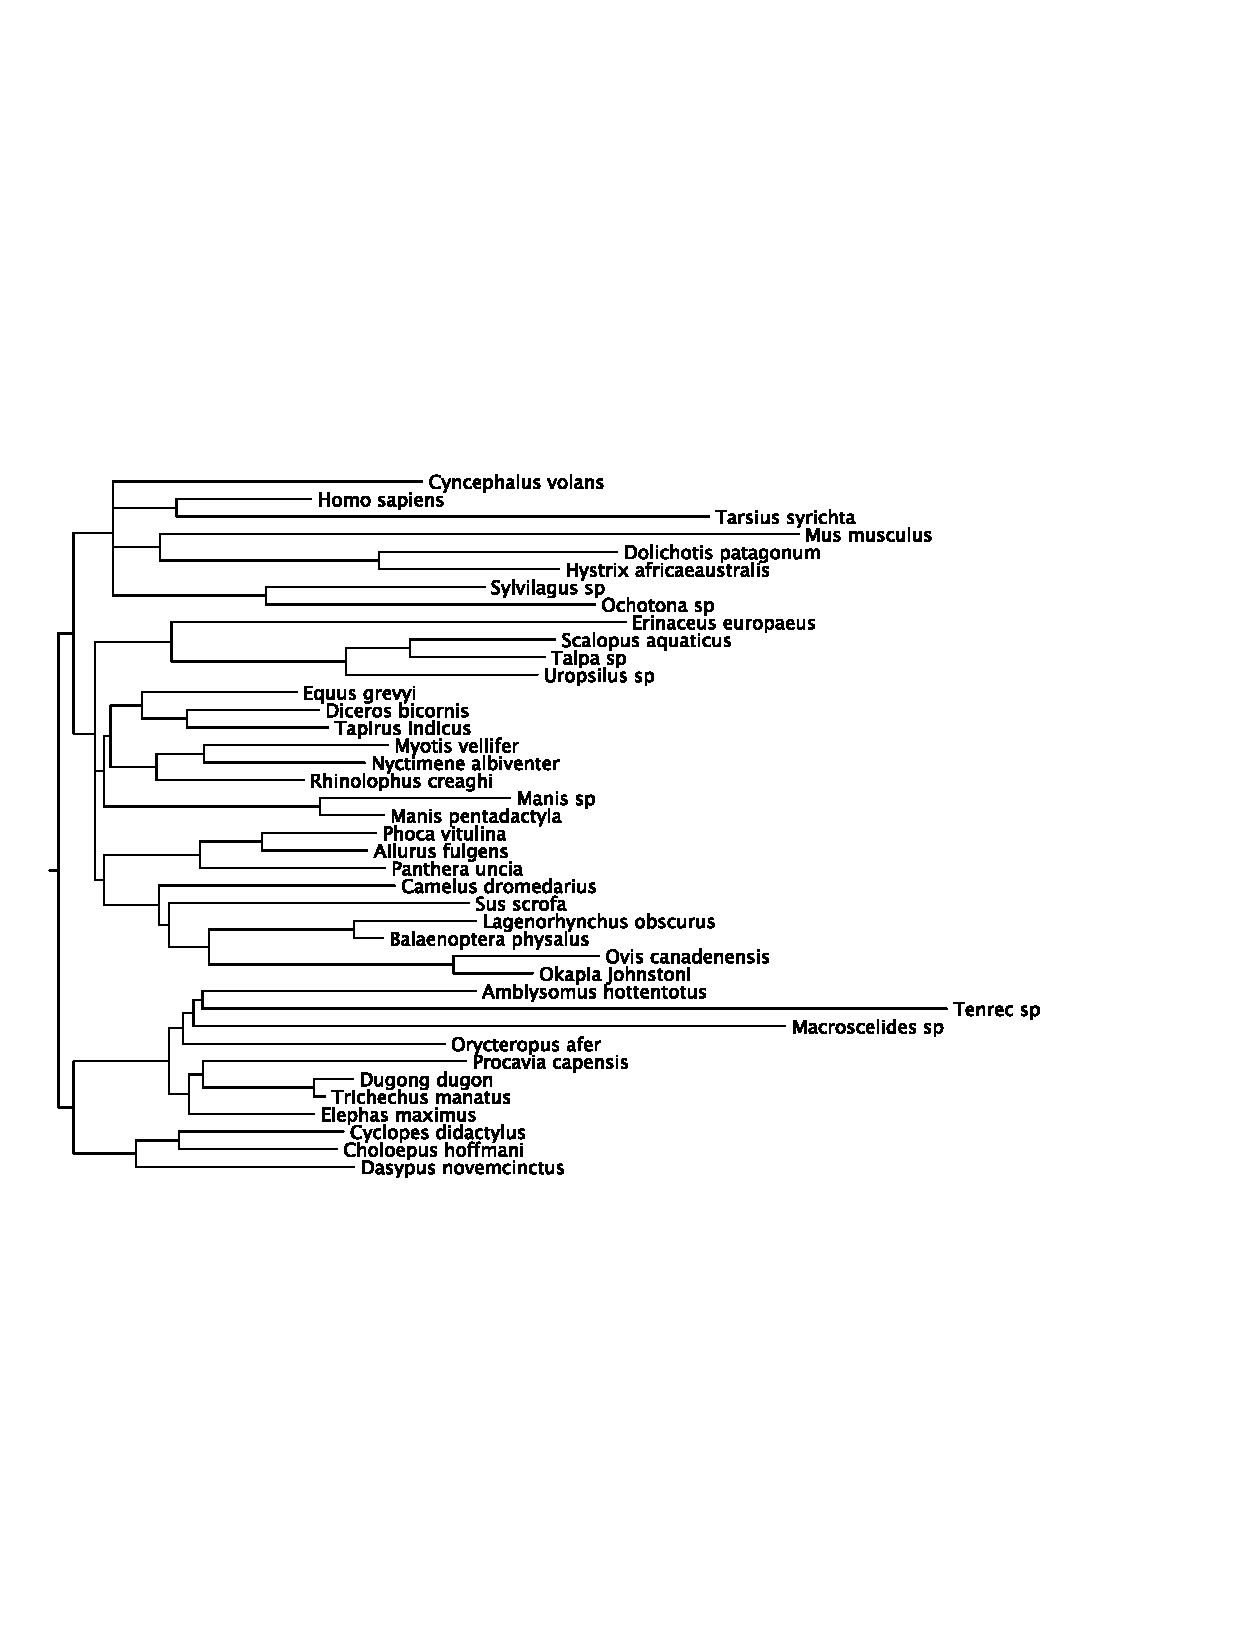
\includegraphics[width=25em]{waddellTree}
	\vskip -.5em
		\caption{Gene tree for RAG-1 sequences used by Waddell {\em et al.~}\citep{WaddellOP2009}. Branch lengths are shown in proportion to the expected number of changes per site. Our algorithm can calculate quantities such as ``the probability of a character evolving on this tree and showing states A and C and a parsimony length of 5''}\label{waddellTreeFig}
	\vskip -1.0em
\end{wrapfigure}
Both the model adequacy assessment \citep{WaddellOP2009} and the extension of Lewis's \citep{Lewis2001} model entail calculations based on classes of patterns that share the same parsimony length on a tree.
The model adequacy test also requires partitioning patterns based on the set of states observed at the leaves of the tree.
Fitch \citep{Fitch1971} provided an efficient algorithm for calculating the parsimony score.
The Fitch algorithm can calculate the parsimony length for a tree rooted at an internal node from a ``downpass state set'' for the children of the node.
We have developed a dynamic programming algorithm that can calculate the probability of class of patterns that share the same set of observed states and parsimony length on a tree.\\
For a tree of $N$ leaves, the algorithm requires storing bins of probability for:
\begin{compactitem}
	\item each of the $N-1$ internal nodes,
	\item each of the $\approx N - 1$ parsimony lengths,
	\item each of the $k$ ancestral states,
	\item  each of the $2^{k}-1$ observed state sets, and
	\item each of the $2^{k}-1$ downpass state sets
\end{compactitem}
yielding an approximate memory requirement of $\mathcal{O}(N^2 k 2^{2k}$).
$k$ is bounded and often small ($k=4$ for DNA data).
With respect to tree size, calculations scale $\mathcal{O}(N^3).$
Waddell {\em et al.~}\citep{WaddellOP2009} used simulation on the tree shown in Figure \ref{waddellTreeFig} to obtain probabilities for classes of patterns.
We validated our algorithm with the same data and confirmed very similar probability calculations (data not shown).
%This figure represents a phylogenetic tree which uses this data to perform pairwise tests.  
}
\headerbox{Specializing for the Symmetric Models}{name=results2,span=2,column=1,below=results}{
\begin{wrapfigure}{r}{15em}
	\vskip -1.5em
		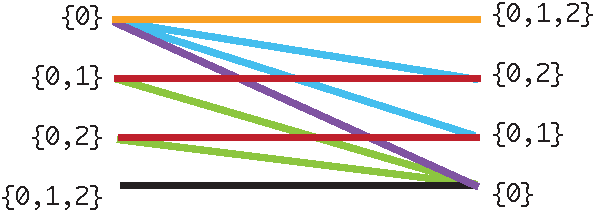
\includegraphics[width=15em]{downpass-symmetry-small}
	\vskip -.5em
	\caption{Combinations of state-sets for left and right child which lead to downpass state set of $\{0\}$ when $k=3$. In the fully symmetric case, edges shown with the same color are guaranteed to have the same probability. There are 9 edges, but only 6 colors.}\label{symmetryFig}
\end{wrapfigure}
We are in the process of developing a specialization of the algorithm for models in which all states are equivalent (such as \citep{Lewis2001}).
Many of the probability calculations return the same answer in these models.
Exploiting the fact that distinct combinations give the same result allows the answer to be calculated with fewer operations. 
We can sketch out a rough computational complexity for a symmetric version of the algorithm.
The exact nature of the observed and downpass state sets do not need to considered.
Rather, we can focus on the size of these sets.  
There are only $k$ distinct sizes (from $1$ to $k$) rather than $2^{k}-1$ state sets.
This unveils the potential for drastic improvement and simplification in the algorithm.\\
{\bf Figure \ref{symmetryFig}} shows a graph representing the calculations required for 
a scenario in which an internal node has the down pass state set of $\{0\}$.
Under a fully symmetric model, the state sets of the same size (e.g. $\{0,1\}$ and $\{0,2\}$) will imply the same probabilities.
While there are 9 combinations of states sets, there are only 6 combinations of state set sizes.
The time savings for this model expand for larger values of $k$.
Applying a symmetric model specialization will enable considerations of characters with many more states.
%There are (n-1) internal nodes in a tree, which increases by a factor of one with each additional leaf on the tree.  (This is scaled linearly).  We must sweep over all the possible parsimony lengths under that, which are equal to [1-(the number of leaves at that point)].  Therefore, at each child we will need to calculate for 0 and 1, whereas at the ancestor we will need to calculate for 0, 1, 2 and 3.  But as the tree becomes very large, the number of calculations / the number of length bins will be approximately of the order n.\\

}
\headerbox{Future Work}{name=results3,column=3,row=0}{
\begin{compactitem}
\item We will continue to optimize the algorithm for the symmetric model to reduce the memory and computational costs.
\item We will test the specializations in software capable of using the general and specialized form of the algorithm.
\item After validating the testing implementation, we will include our approaches in the GARLI \citep{GARLI} software package, which is a widely-used software tool for inferring evolutionary trees.  
\item We will add calculation of goodness-of-fit statistics from the probabilities that our algorithms compute. 
This will constitute an implementation of the method of Waddell {\em et al.~}\citep{WaddellOP2009} which can be used to assess model adequacy on large phylogenetic trees.
Assessing models of character evolution on large trees provides a more rigorous test of model adequacy.
\end{compactitem}
This work is being conducted according to the principles of open notebook science; all software, notes, and results are
publicly viewable on \url{https://github.com/mtholder/PhyPatClassProb}
}

\headerbox{Acknowledgements}{name=acknowledgements,column=3,below=results3}{
\smaller						% Make the whole text smaller
\vspace{-0.4em}			% Save some space at the beginning
We would like to thank NIH 5 R25GM62232 and the Initiative for Maximizing Student Diversity for funding.
} 

\headerbox{References}{name=references,column=3,below=acknowledgements}{
\smaller													% Make the whole text smaller
\vspace{-0.4em} 										% Save some space at the beginning
\bibliographystyle{plain}							% Use plain style
\renewcommand{\section}[2]{\vskip 0.05em}		% Omit "References" title
\bibliography{../pattern_class}
}



\end{poster}
\end{document}
